%
% file: localoperator.tex
% author: Victor Brena
% description: Briefly describes properties of the local operator.
%

\chapter{AADH}\label{app:aadh}
\begin{figure}[p]
    \centering
    \mycaption{LOW RESOLUTION! RMSD of the $\alpha$-Carbon atoms of AADH relative to the crystal structure. Each panel is a single trajectory, blue lines are the RMSD, black horizontal lines are the \SI{2.5}{\percent} and \SI{97.5}{\percent} quantiles (\SI{4.5}{\angstrom} and \SI{6.4}{\angstrom}, respectively) taken across all trajectories.}
    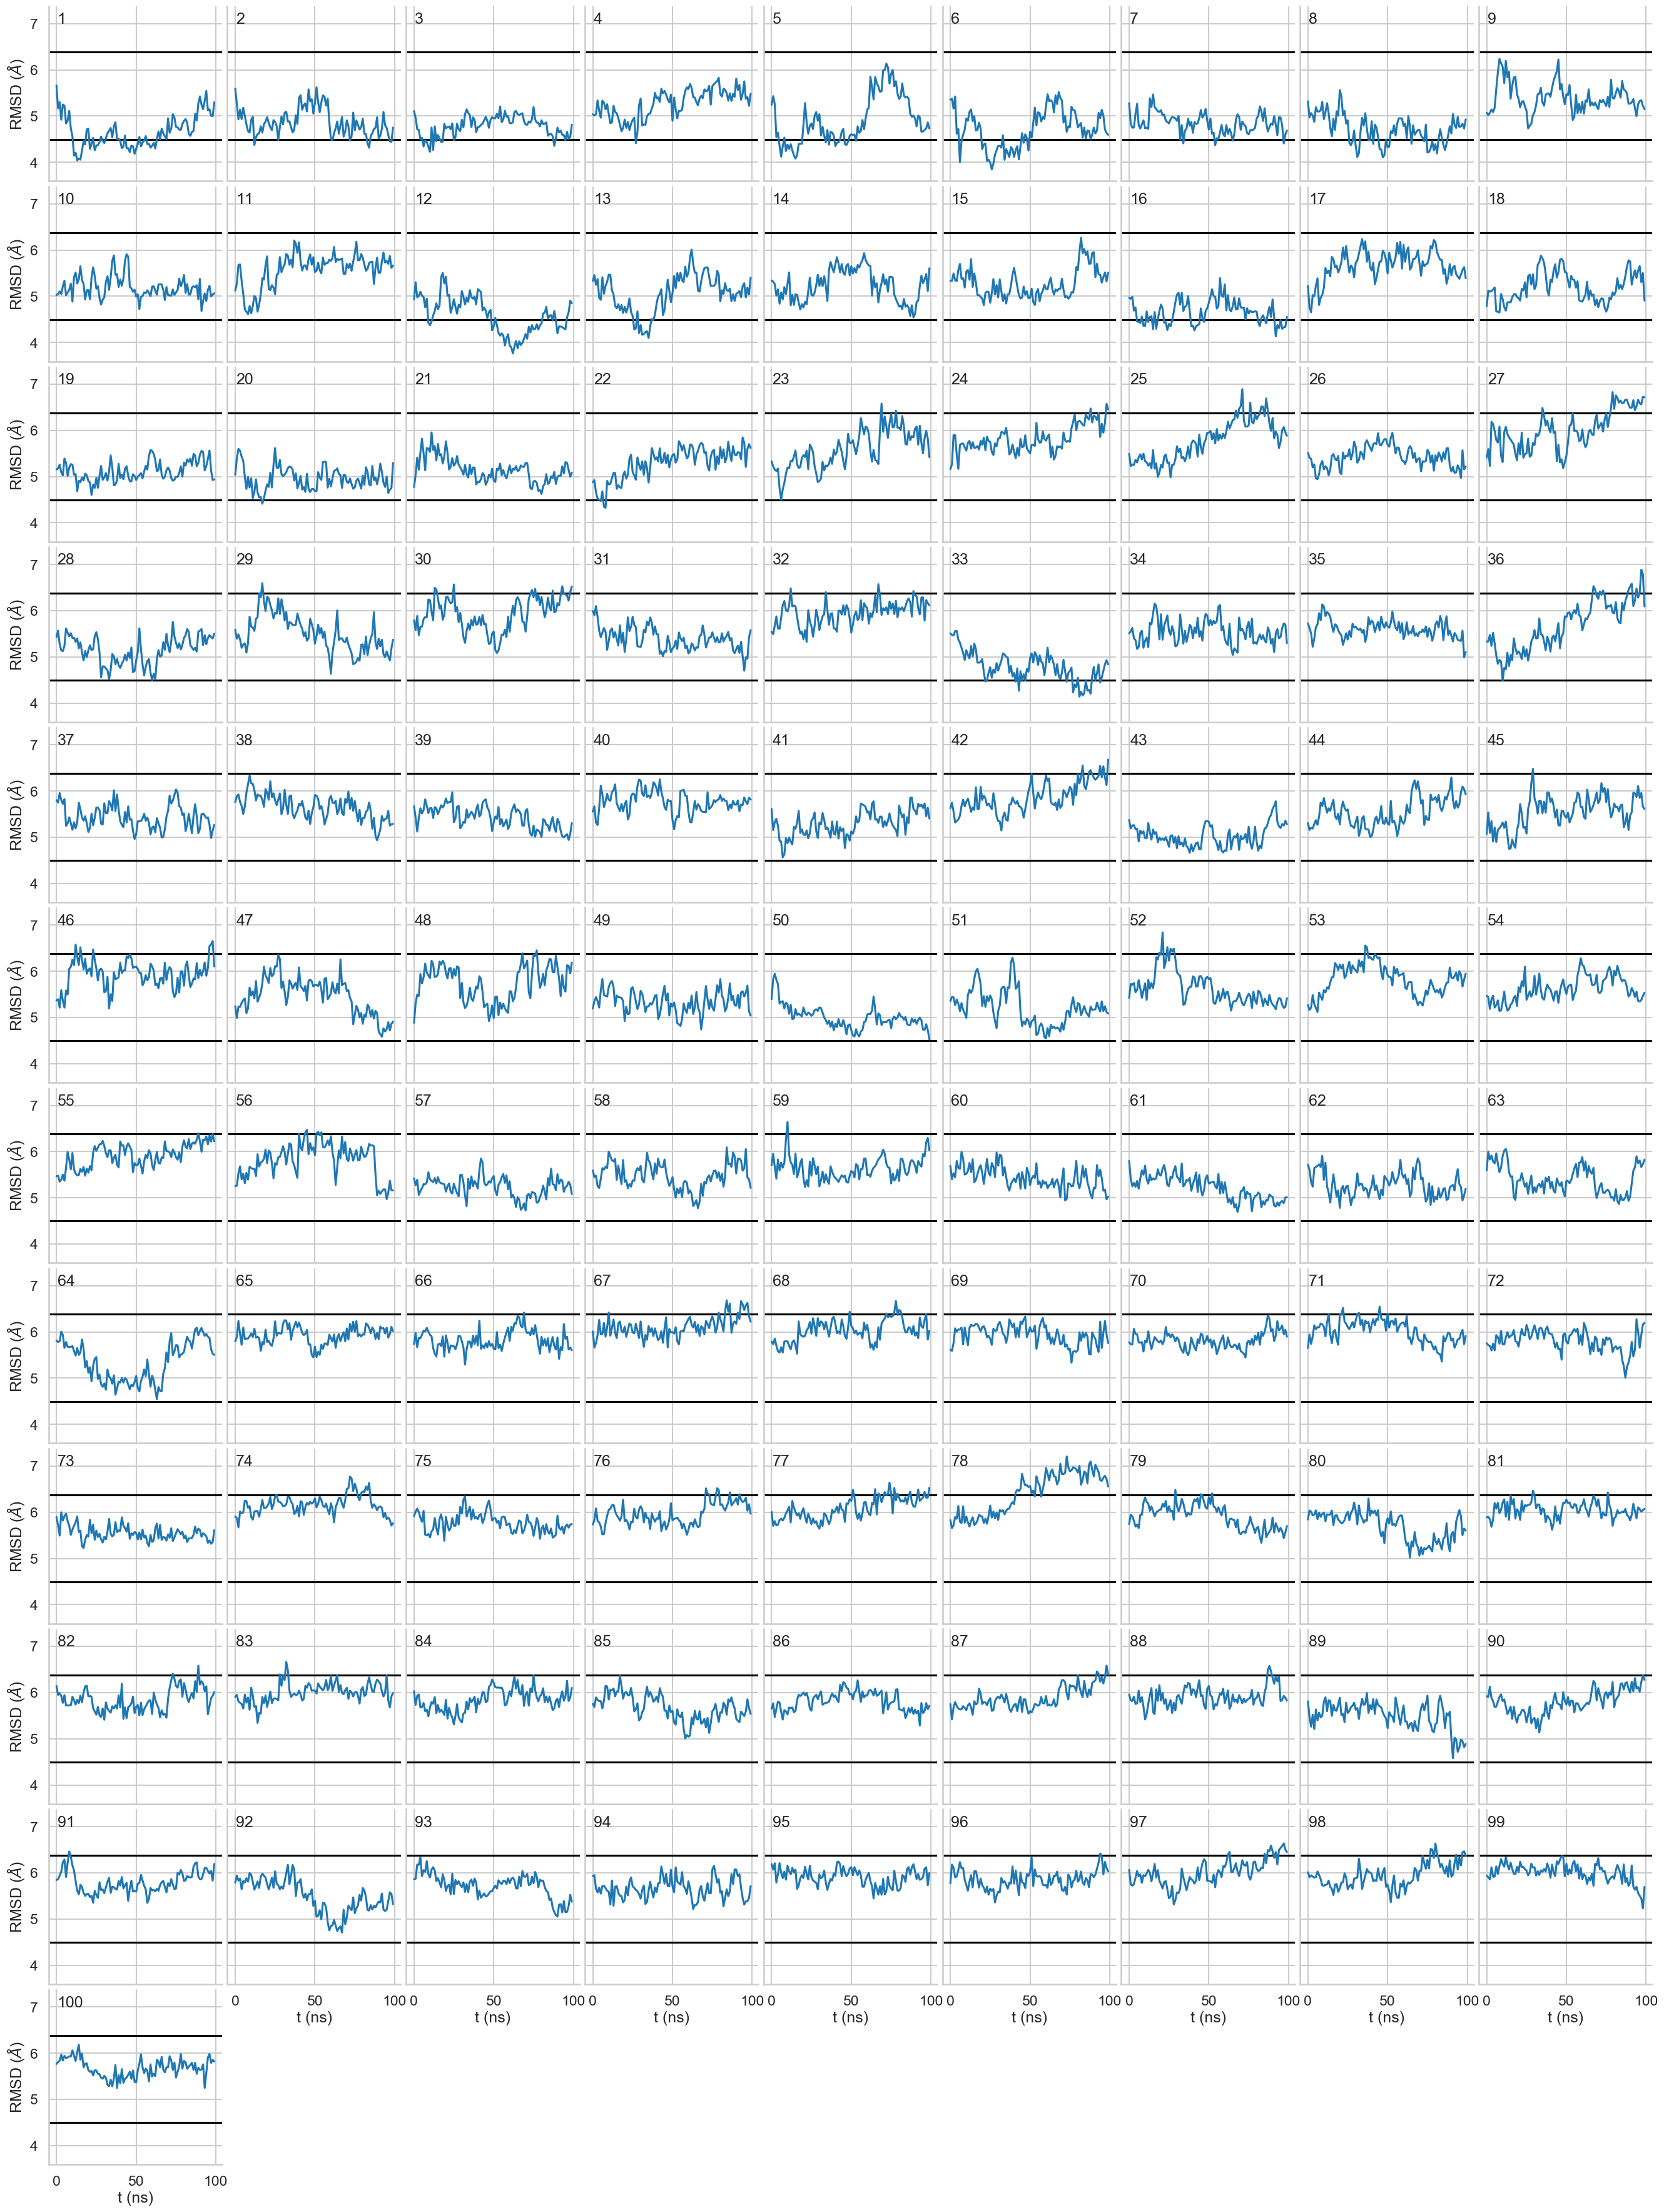
\includegraphics[width=0.9\textwidth]{chapters/aadh/figures/rmsd_backbone_ca.png}
    \label{fig:rmsd_ca}
\end{figure}

\begin{figure}
    \centering
    \mycaption{Secondary structure composition of trajectories $24, 27, 30, 42, 78, 87$ and $97$ as a function of time. The number of residues in each simplified secondary structure class \cite{kabschDictionaryProteinSecondary1983} are shown: `H' (green) refers to alpha helix, 3- and 5-helices; `E' (orange) refers to residues in beta-bridges or  beta ladder; `C' (blue) refers to turns, bends and all irregular elements.}
    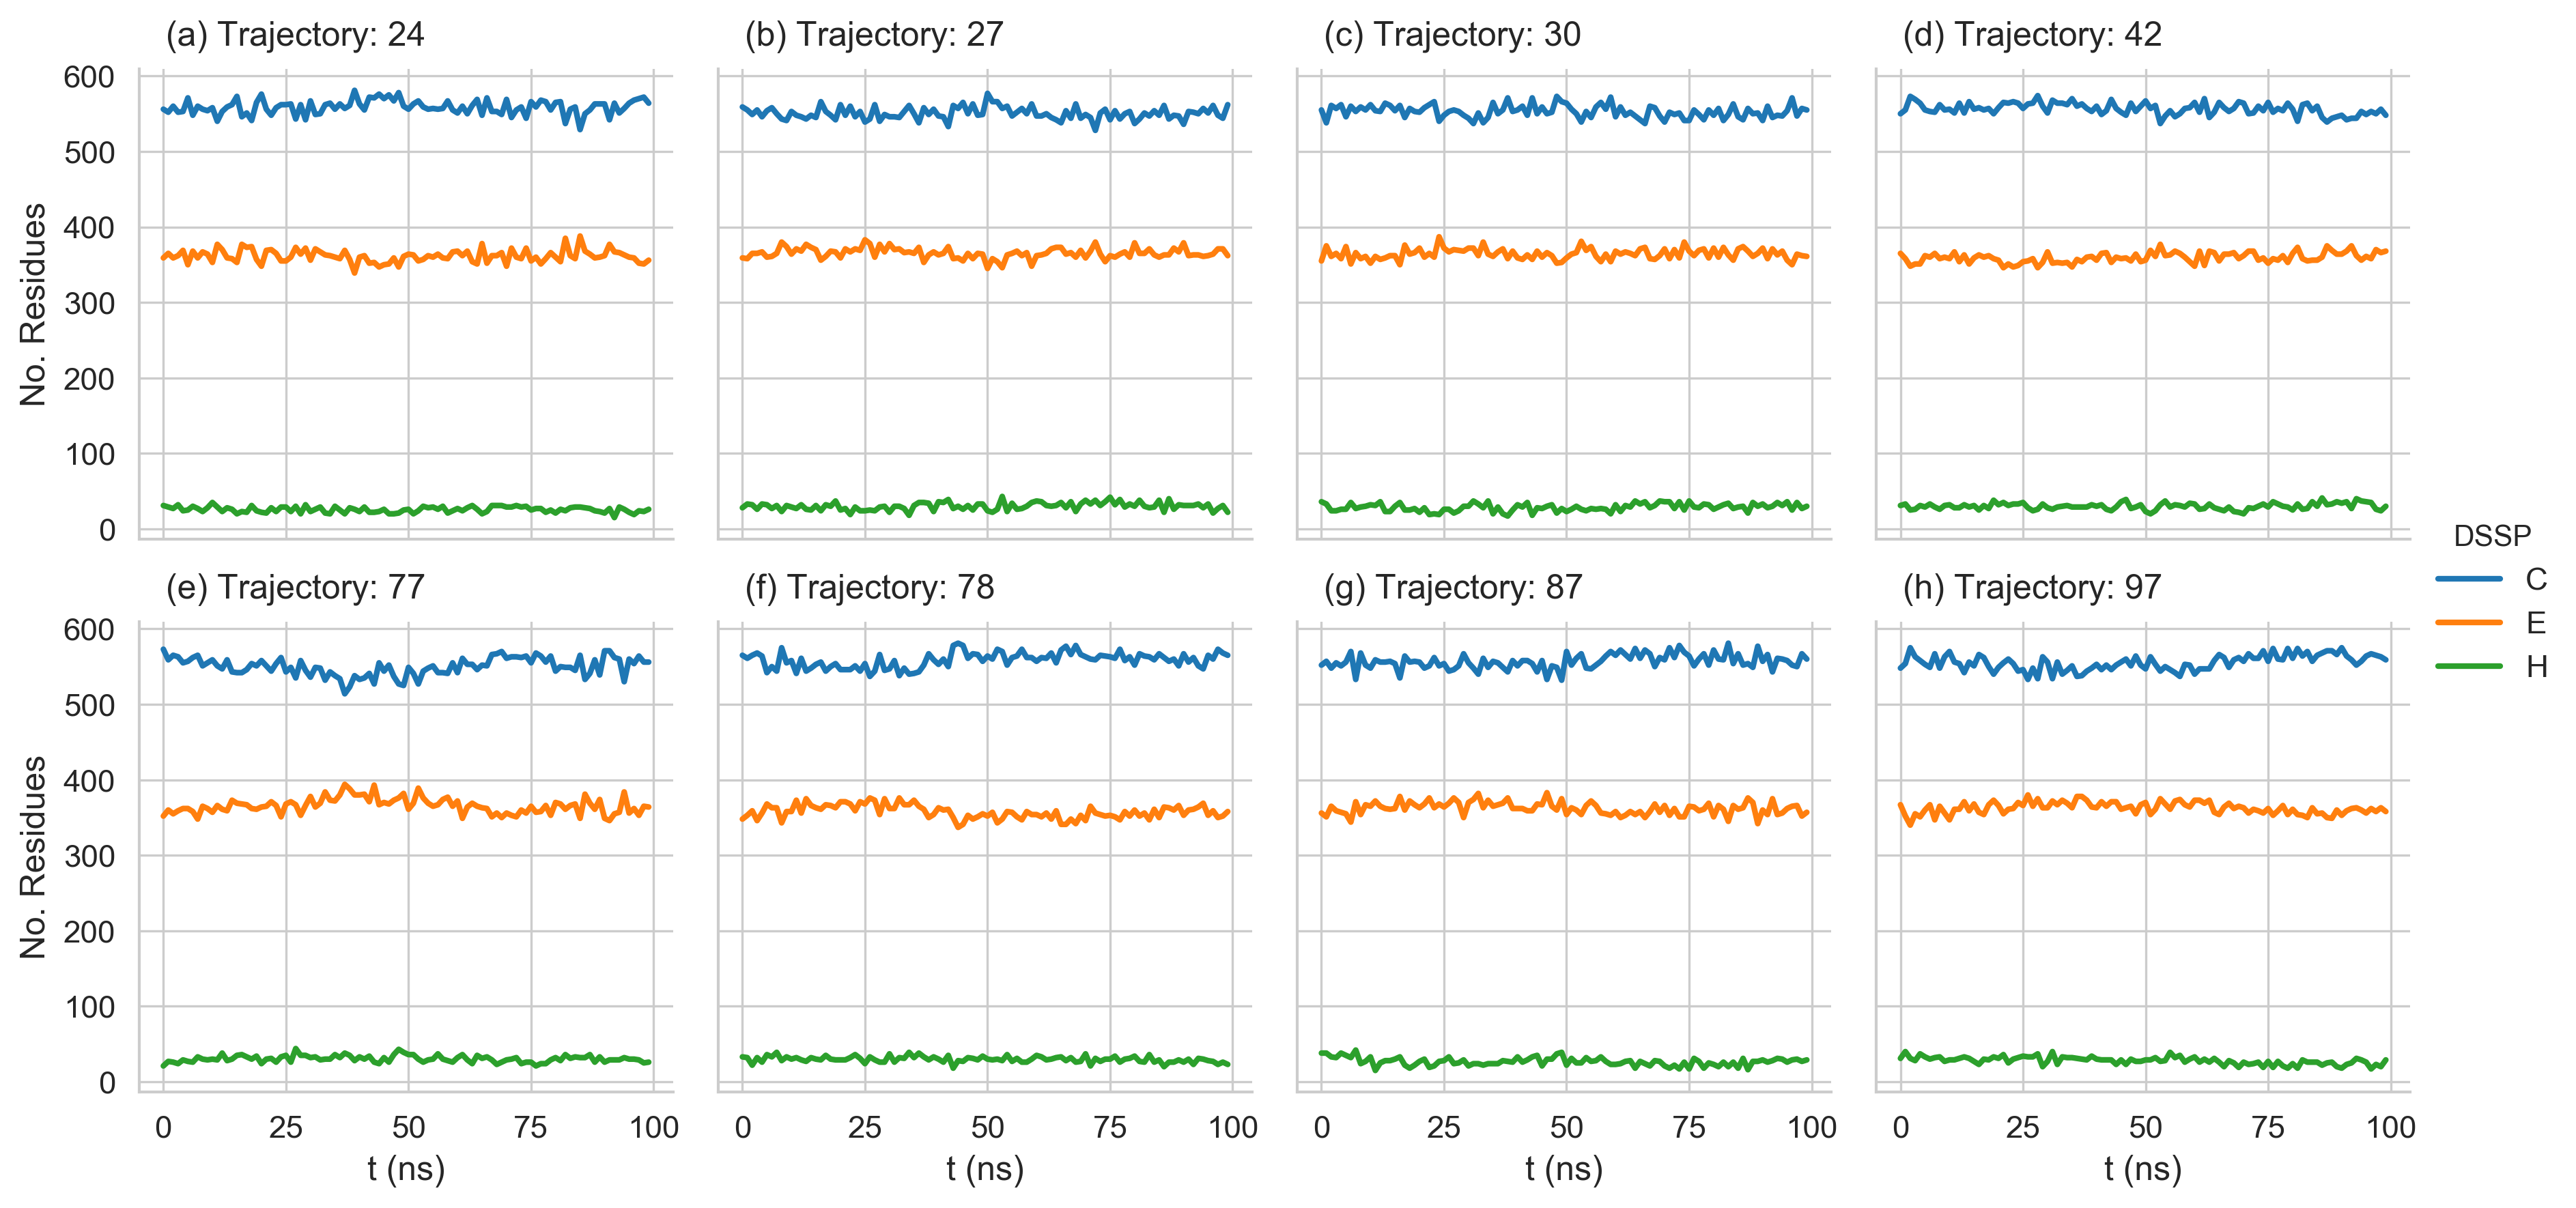
\includegraphics[width=0.9\textwidth]{chapters/aadh/figures/drift_trajs_dssp.png}
    \label{fig:dssp_trajs_sens}
\end{figure}

\begin{figure}
    \centering
    \mycaption{The ratio of successive implied timescales for a Markov state model with $\tau(\textrm{MSM})=\SI{2}{\nano\second}$ estimated using MCMC with $1000$ posterior samples. The TICA lag time was set to $\tau=\SI{10}{\nano\second}$, with \SI{95}{\percent} of the variance retained meaning $m=8$ components were retained. The number of cluster centres was set to $n=316$. The blue dots and error bars are the mean and \SI{95}{\percent} credible intervals.}
    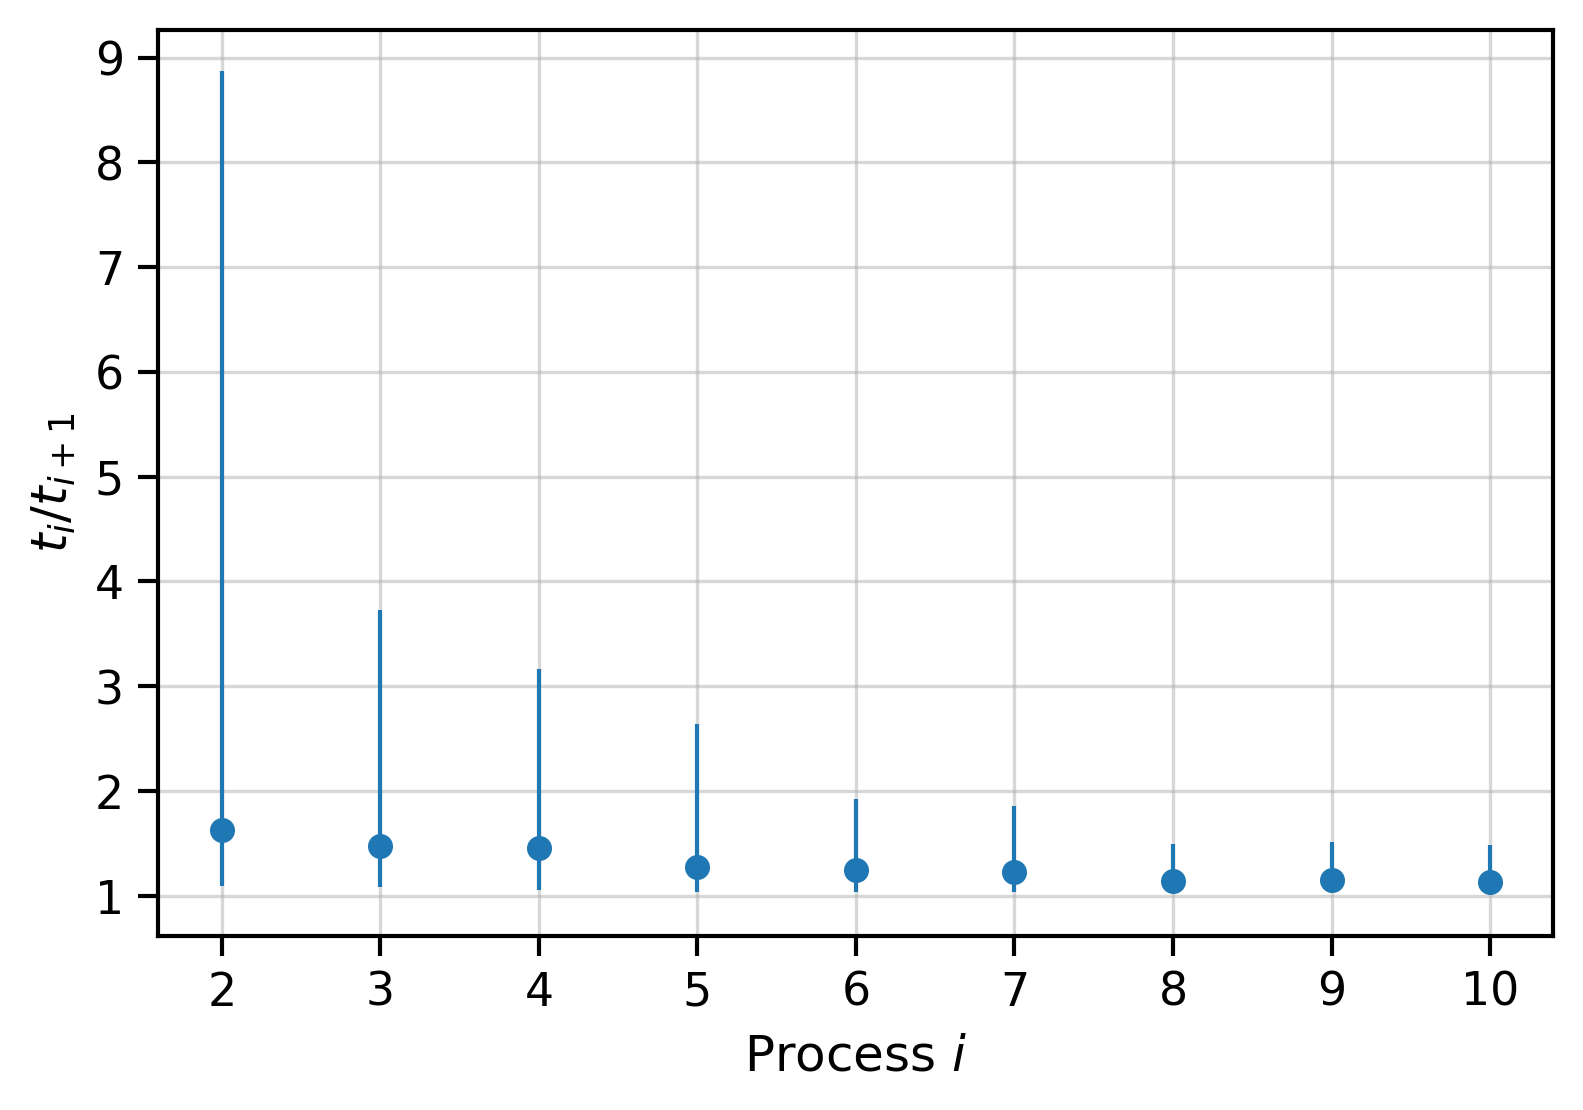
\includegraphics[width=0.8\textwidth]{chapters/aadh/figures/timescale_ratios_D_sens.png}
    \label{fig:ts_ratios_d_sens}
\end{figure}

\begin{figure}
    \centering
    \mycaption{The implied timescales and relative VAMP-2 scores as a function of the Markov lag time $\tau(\mathrm{MSM})$. The TICA lag time was set to $\tau=\SI{10}{\nano\second}$, with \SI{95}{\percent} of the variance retained meaning $m=8$ components were retained. The number of cluster centres was set to $n=316$. Panel (a) shows the first five implied timescales for $\SI{0}{\nano\second} < \tau(\mathrm{MSM}) < \SI{5}{\nano\second}$, panel (b) shows the first five implied timescales for $\SI{0}{\nano\second} < \tau(\mathrm{MSM}) < \SI{50}{\nano\second}$. The solid lines and coloured shaded areas are the mean and \SI{95}{\percent} credible intervals respectively, estimated using MCMC with $500$ posterior samples. The grey shaded area is the region for which the implied timescales are smaller than the lag time. Panel (c) and (d) show the VAMP-2 scores, scored on the first $2-5$ eigenvalues for the same ranges. The VAMP-2 scores are indexed to $1$ at their initial value. The colour coding is consistent between the implied timescale plots and VAMP-2 plots. So that $k=2$, in blue, is the score including the first eigenvalue $\lambda = 1$ and the eigenvalue of the longest implied timescale also shown in blue in panels (a) and (b). }
    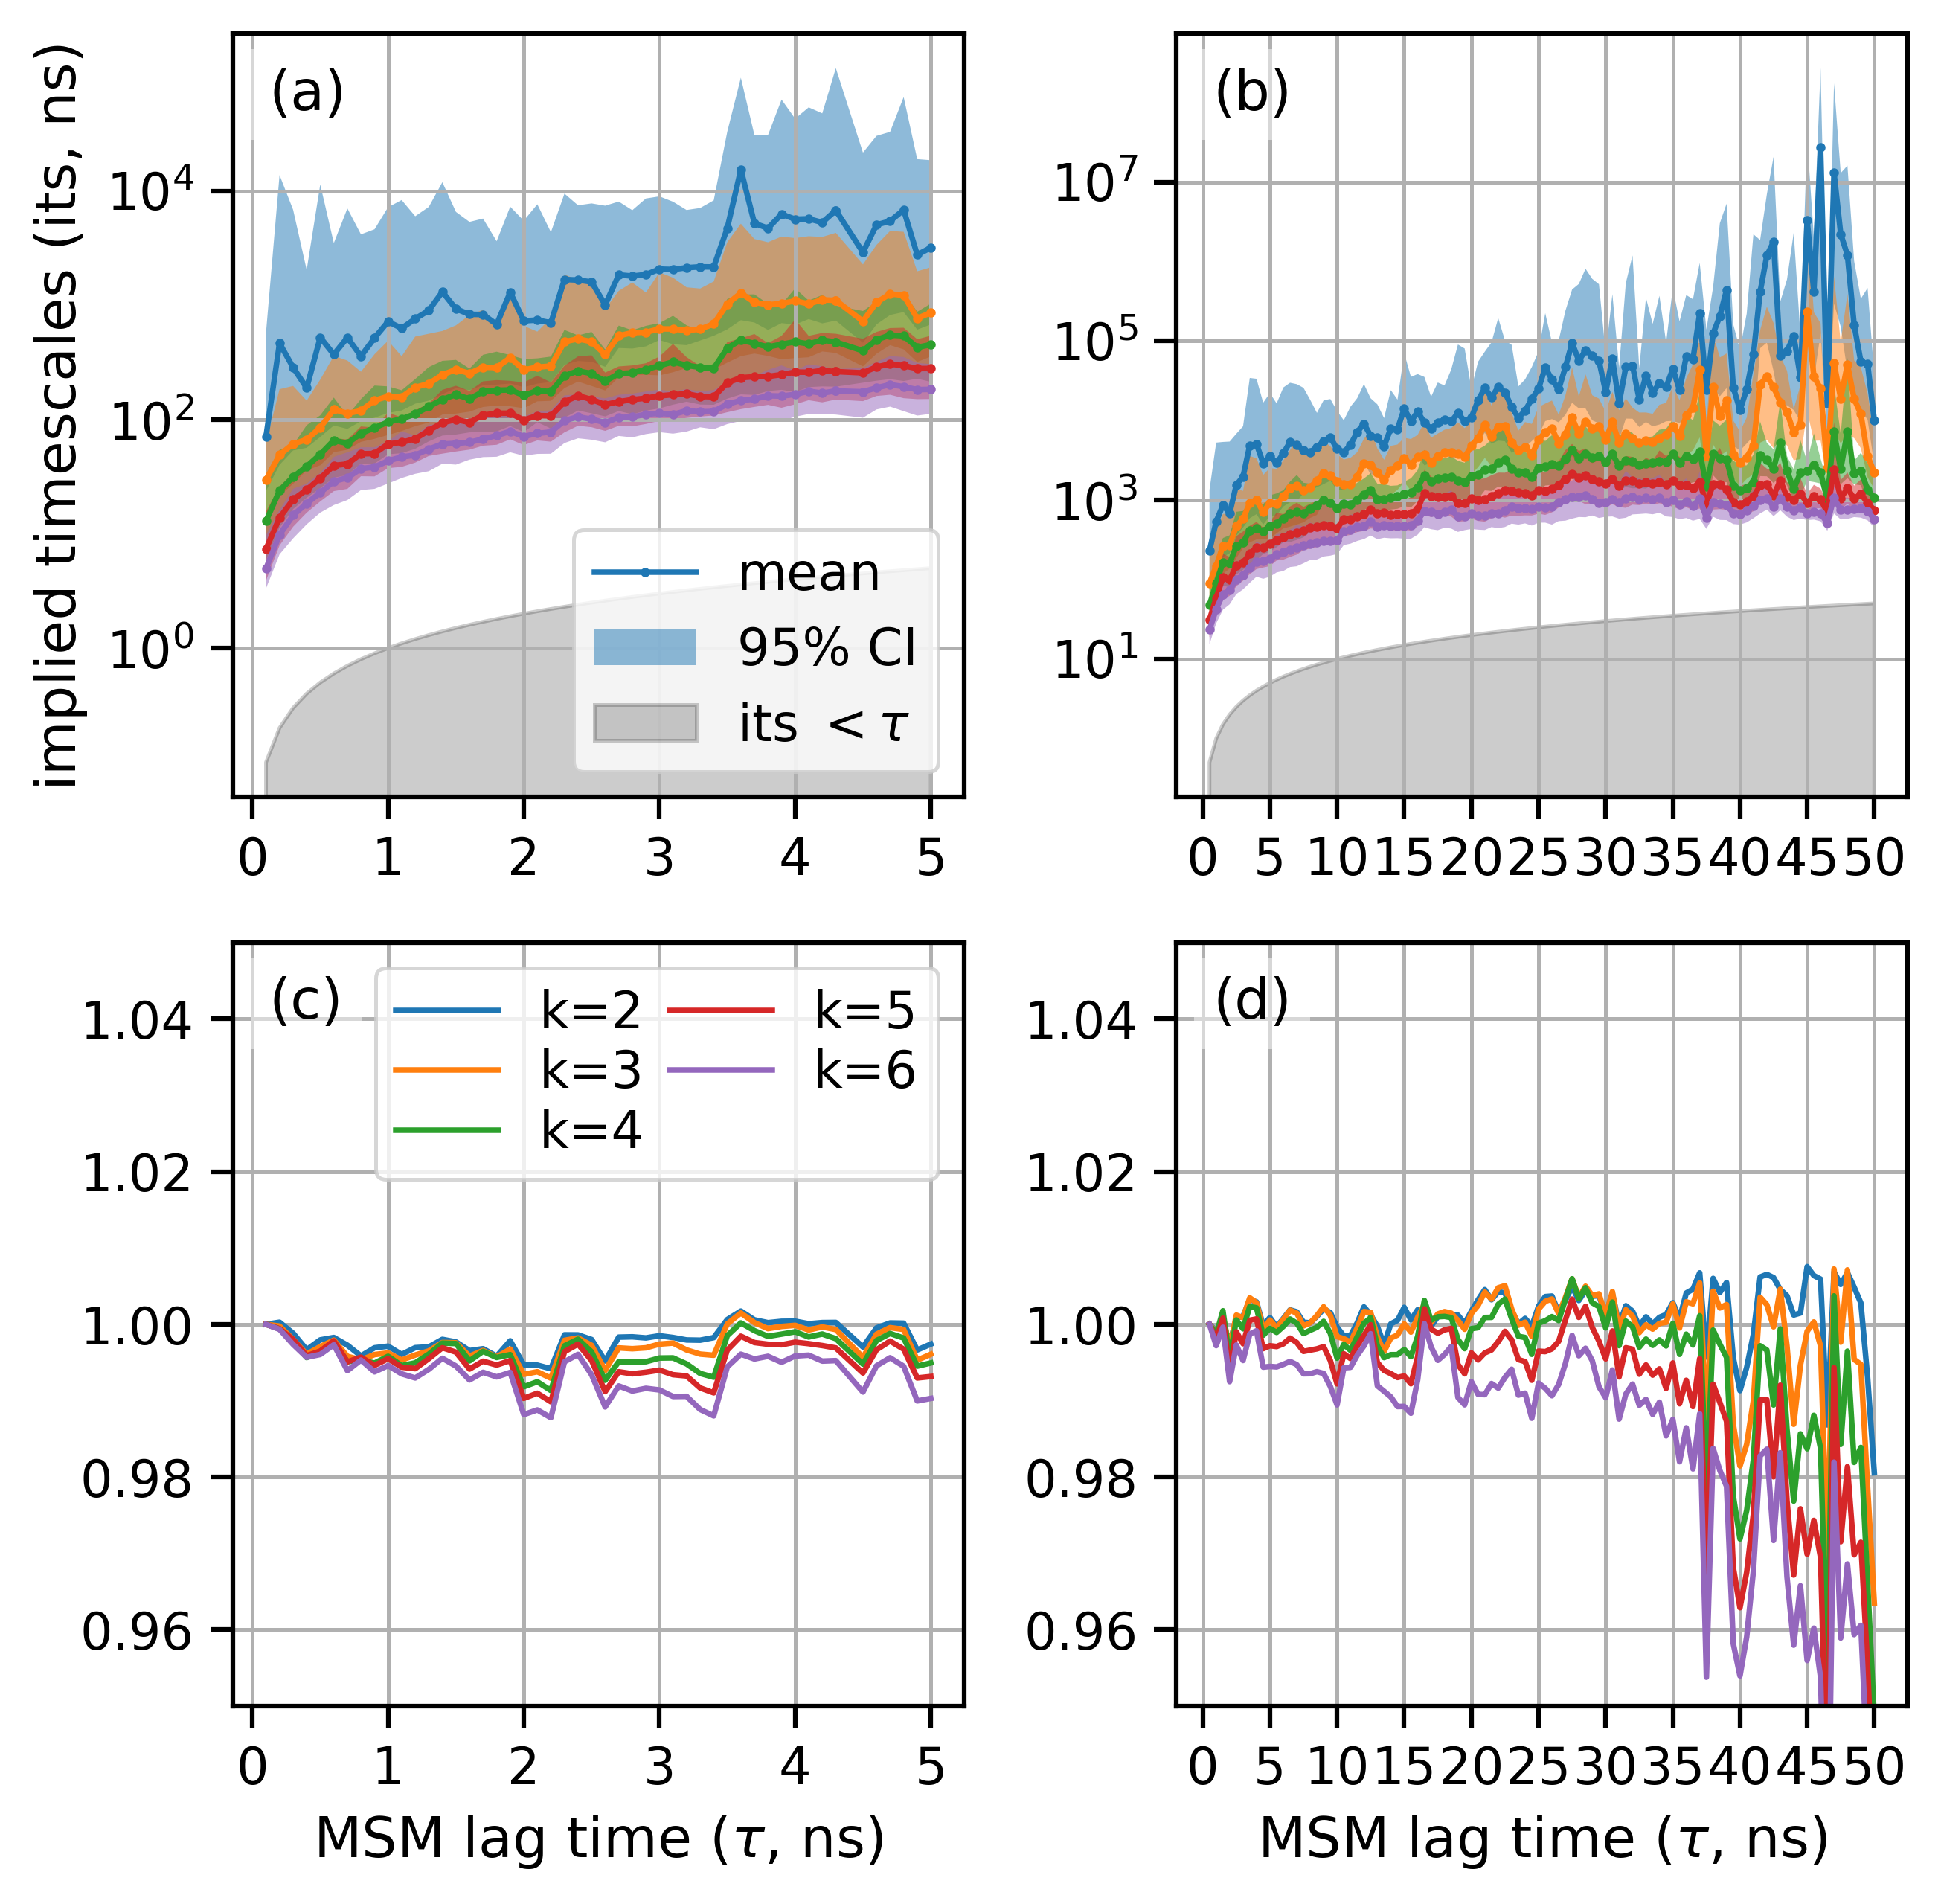
\includegraphics[width=0.8\textwidth]{chapters/aadh/figures/implied_timescales_D_sens.png}
    \label{fig:its_d_sens}
\end{figure}



\chapter{MSM optimisation}\label{app:msm}

\section{Alanine Dipeptide}

\begin{table}[h]
    \centering
    \caption{ Model selection metrics othe response surface of Alanine Dipeptide. Standardised mean square error (SMSE) and mean standardised log loss (MSLL) for GP models of the response surface of MSMs for alanine dipeptide, using different transformations of $n$ ($T(n)$) and different kernels. Each GP model used a mean prior of zero, and all other parameters were estimated by maximizing the marginal likelihood. All values were calculated using 10-fold cross-validation.}
    \begin{tabular}{|l|l|c|c|c|}
    \hline
    T(n) &       Name &  SMSE &    MSLL \\
    \hline\hline
     $\log{(n)}$ &  Exponential & 0.0012 & -3.9963 \\
      &  Mat{\'e}rn 3-2  & 0.0010 & -4.1712 \\
      &  Mat{\'e}rn 5-2  & 0.0007 & -4.2369 \\
      &  Gaussian & 0.0011 & -4.0892 \\
     $I(n)$ &  Exponential  & 0.0027 & -2.9733 \\
      &  Mat{\'e}rn 3-2  & 0.0025 & -3.4218 \\
      &  Mat{\'e}rn 5-2  & 0.0023 & -3.8172 \\
      &  Gaussian & 0.0032 & -4.1239 \\
    \hline
    \end{tabular}
    \label{tab:ala2_fit_results}
\end{table}

% \begin{figure}
%     \centering
%     \caption{Caption}
%     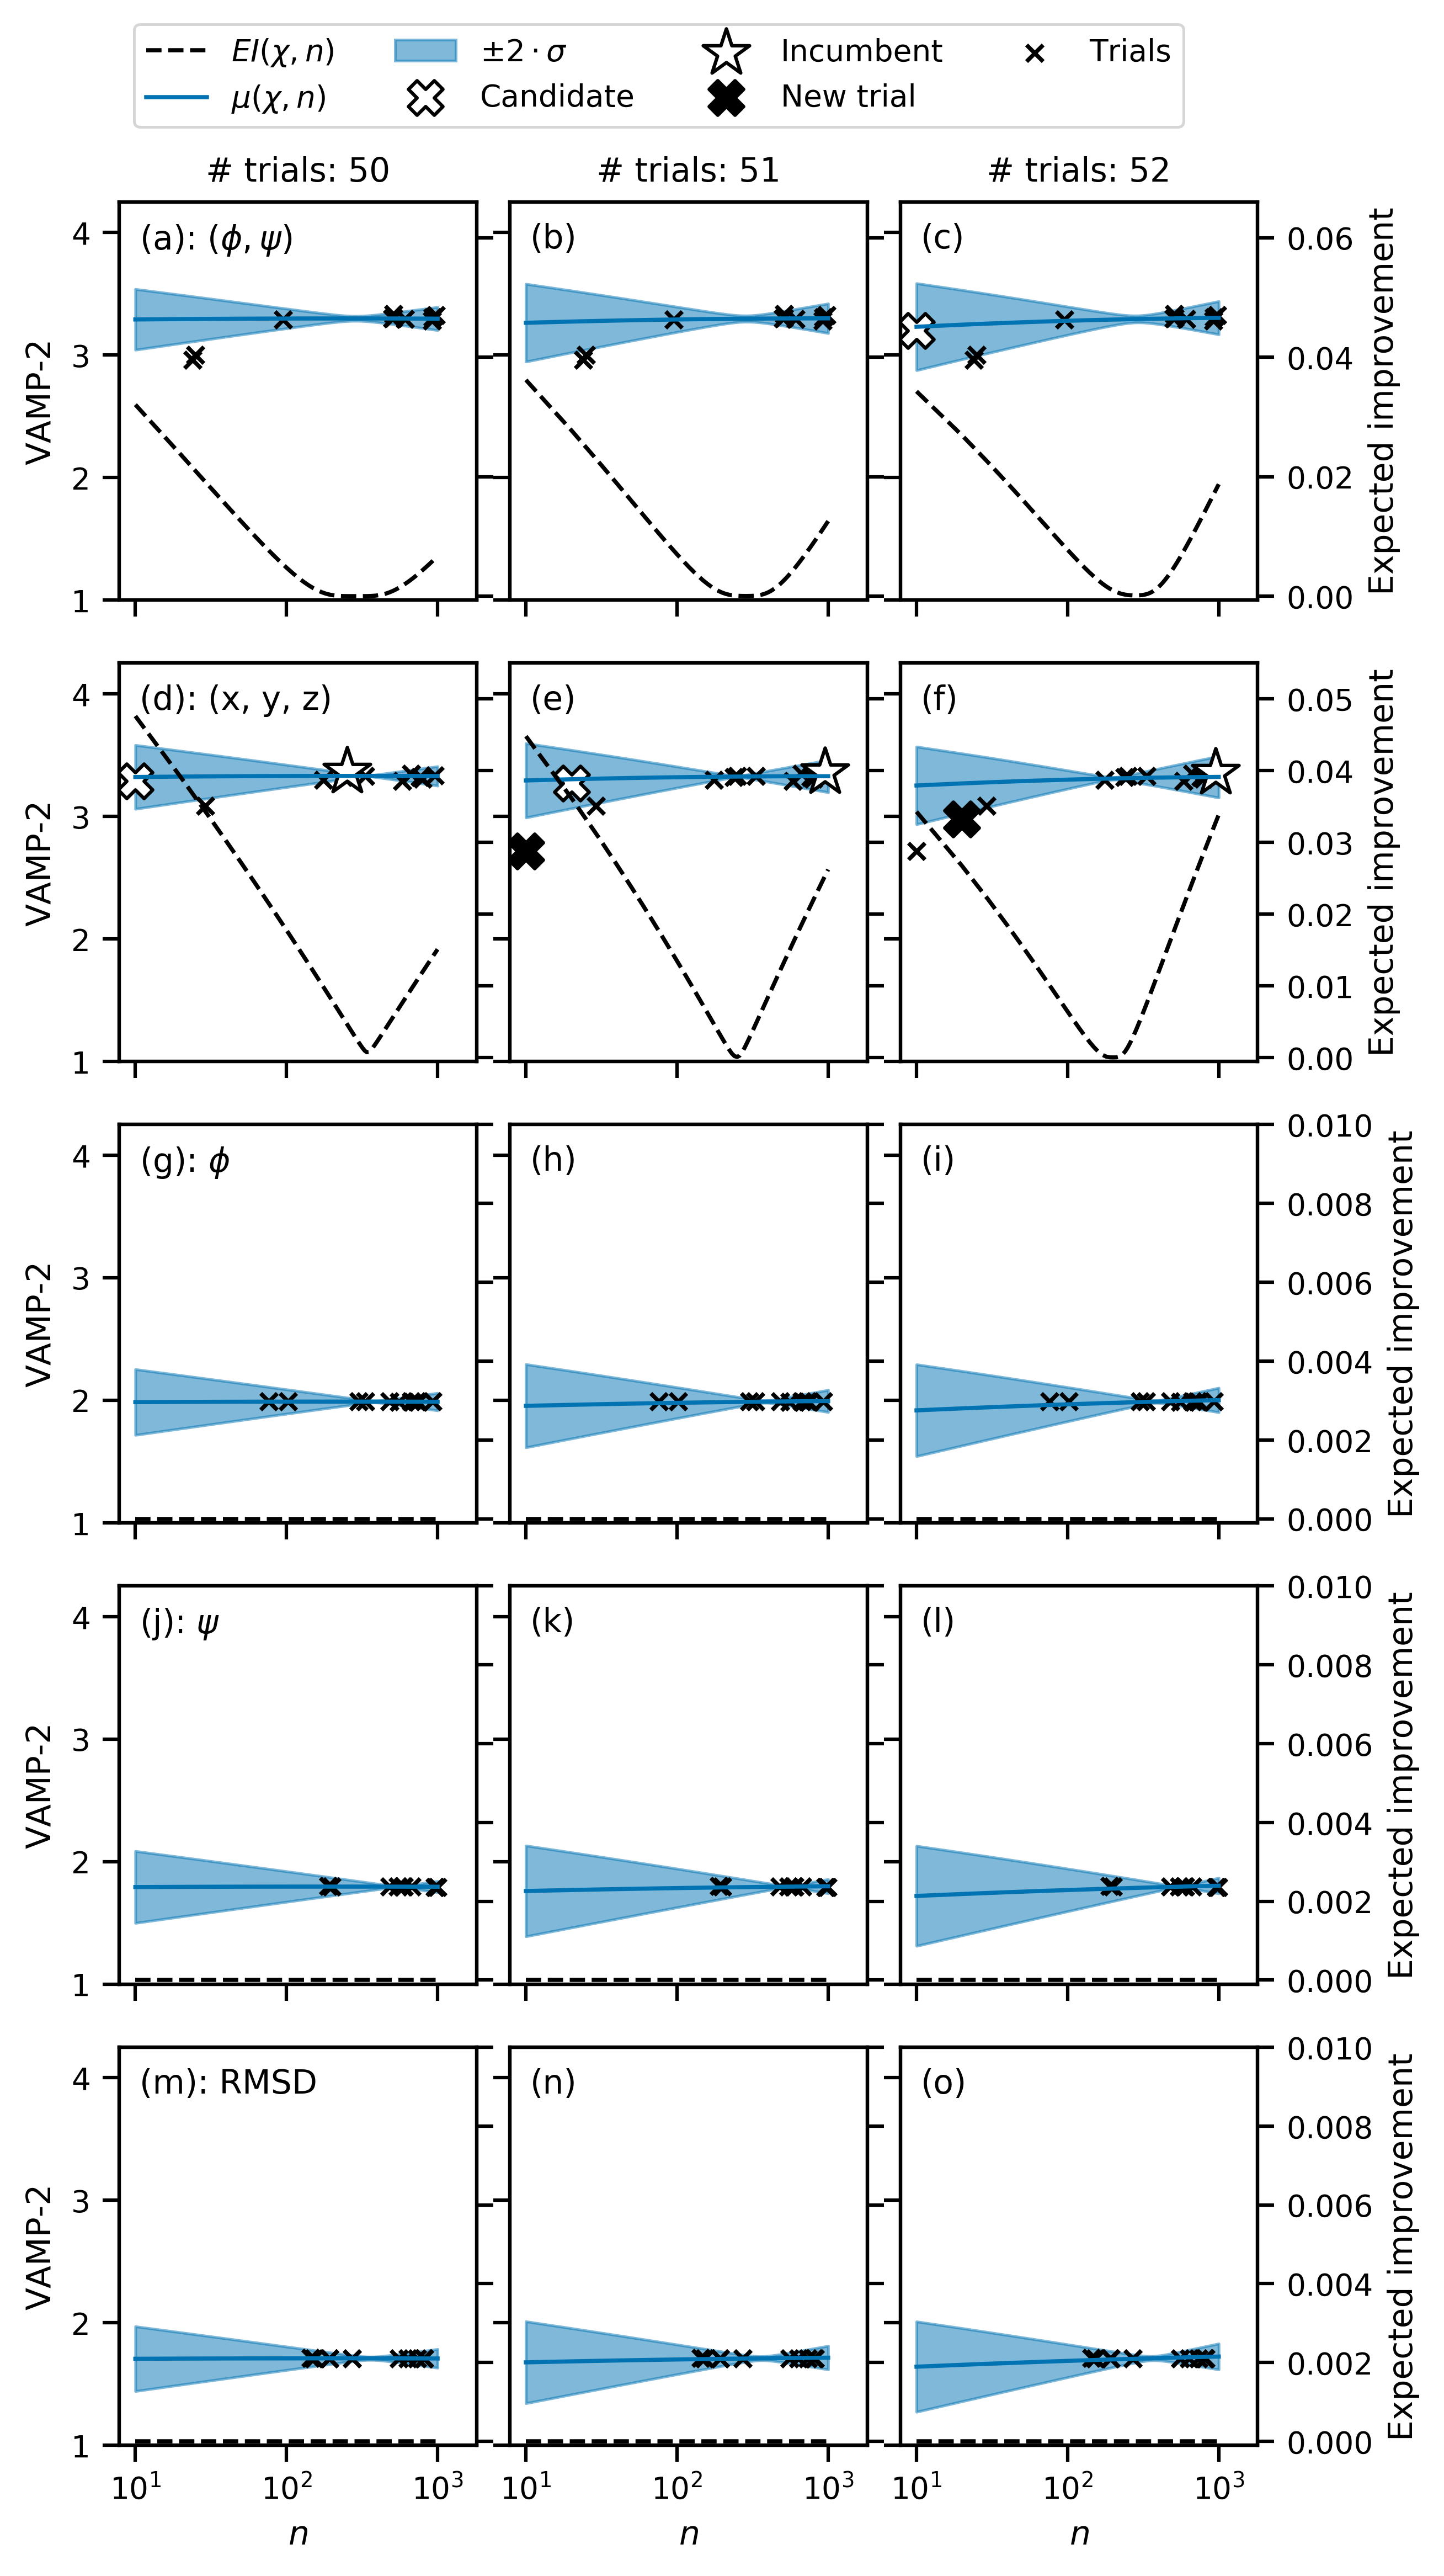
\includegraphics[height=0.8\textheight]{chapters/msm_optimization/figures/ala1_opt_explainer.png}
%     \label{fig:ala1_opt_expl}
% \end{figure}

\section{AADH}

\begin{table}
    \centering
    \caption{Model selection metrics for the response surface of AADH using all hyperparameter trials ($N=361$, except those for $\chi=$RMSD). The Mean Standardised Log Loss (MSLL) and Standardised Mean Square Error (SMSE) where calculated using 10 fold cross validation. Only those models which had both $\mathrm{MSLL}<0$ and $\mathrm{SMSE}<1$ were ranked. The total rank is calculated as rank of $\sqrt{R_{MSLL}^{2}+R_{SMSE}^2}$. Where the overall rank was tied, the first model appearing in the table was ranked higher. }
    \label{tab:aadh_rsm_metrics_all_data}
    \begin{tabularx}{1\textwidth}{|llllrr >{\raggedright\arraybackslash}X>{\raggedright\arraybackslash}X>{\raggedright\arraybackslash}X|}
    \hline
    $T(\tau)$ & $T(m)$ & $T(n)$ & Kernel & MSLL &   SMSE & Rank (MSLL) & Rank (SMSE) & Rank (Total)\\
    \hline\hline
    $I({\tau})$ & $I({m})$ & $I({n})$ & Exponential & -0.1298 & 0.3087 &       1.0 &       1.0 &  1.0 \\
                   &             & $\log({n})$ & Exponential &  0.0050 & 0.2964 &         - &         - &    - \\
                   & $\log({m})$ & $I({n})$ & Exponential &  0.0521 & 0.3118 &         - &         - &    - \\
                   &             & $\log({n})$ & Exponential &  0.5633 & 0.3815 &         - &         - &    - \\
    $\log({\tau})$ & $I({m})$ & $I({n})$ & Exponential &  0.1967 & 0.3436 &         - &         - &    - \\
                   &             & $\log({n})$ & Exponential &  0.4959 & 0.3231 &         - &         - &    - \\
                   & $\log({m})$ & $I({n})$ & Exponential &  0.5128 & 0.4365 &         - &         - &    - \\
                   &             & $\log({n})$ & Exponential &  1.0267 & 0.4201 &         - &         - &    - \\
    $I({\tau})$ & $I({m})$ & $I({n})$ & M32 &  1.5680 & 0.2893 &         - &         - &    - \\
                   &             & $\log({n})$ & M32 &  1.9193 & 0.2960 &         - &         - &    - \\
                   & $\log({m})$ & $I({n})$ & M32 &  3.1385 & 0.2775 &         - &         - &    - \\
                   &             & $\log({n})$ & M32 &  2.0358 & 0.2818 &         - &         - &    - \\
    $\log({\tau})$ & $I({m})$ & $I({n})$ & M32 &  6.9015 & 0.3203 &         - &         - &    - \\
                   &             & $\log({n})$ & M32 &  7.7182 & 0.3406 &         - &         - &    - \\
                   & $\log({m})$ & $I({n})$ & M32 &  7.9209 & 0.3257 &         - &         - &    - \\
                   &             & $\log({n})$ & M32 &  3.0002 & 0.3472 &         - &         - &    - \\
    $I({\tau})$ & $I({m})$ & $I({n})$ & M52 &  3.6517 & 0.3029 &         - &         - &    - \\
                   &             & $\log({n})$ & M52 &  3.8316 & 0.3090 &         - &         - &    - \\
                   & $\log({m})$ & $I({n})$ & M52 &  8.6574 & 0.2991 &         - &         - &    - \\
                   &             & $\log({n})$ & M52 &  3.7354 & 0.3238 &         - &         - &    - \\
    $\log({\tau})$ & $I({m})$ & $I({n})$ & M52 &  8.9207 & 0.3679 &         - &         - &    - \\
                   &             & $\log({n})$ & M52 & 11.8753 & 0.4064 &         - &         - &    - \\
                   & $\log({m})$ & $I({n})$ & M52 & 12.7637 & 0.3722 &         - &         - &    - \\
                   &             & $\log({n})$ & M52 & 13.6735 & 0.3475 &         - &         - &    - \\
    $I({\tau})$ & $I({m})$ & $I({n})$ & RBF &     inf &    inf &         - &         - &    - \\
                   &             & $\log({n})$ & RBF &  9.3618 & 0.3256 &         - &         - &    - \\
                   & $\log({m})$ & $I({n})$ & RBF &  5.9123 & 0.3022 &         - &         - &    - \\
                   &             & $\log({n})$ & RBF &     inf &    inf &         - &         - &    - \\
    $\log({\tau})$ & $I({m})$ & $I({n})$ & RBF & 17.4786 & 0.4551 &         - &         - &    - \\
                   &             & $\log({n})$ & RBF & 16.7568 & 0.3556 &         - &         - &    - \\
                   & $\log({m})$ & $I({n})$ & RBF & 16.7412 & 0.5026 &         - &         - &    - \\
                   &             & $\log({n})$ & RBF & 24.3199 & 0.4986 &         - &         - &    - \\
    \hline
    \end{tabularx}
\end{table}




\begin{table}
    \centering
    \caption{Model selection metrics for the response surface of an MSM of AADH, data subset 1, $N=100$, except those for $\chi=$RMSD). The Mean Standardised Log Loss (MSLL) and Standardised Mean Square Error (SMSE) where calculated using 10 fold cross validation. Only those models which had both $\mathrm{MSLL}<0$ and $\mathrm{SMSE}<1$ were ranked. The total rank is calculated as rank of $\sqrt{R_{MSLL}^{2}+R_{SMSE}^2}$. Where the overall rank was tied, the first model appearing in the table was ranked higher. }
    \label{tab:aadh_rsm_metrics_iter_1}
    \begin{tabularx}{1\textwidth}{|llllrr >{\raggedright\arraybackslash}X>{\raggedright\arraybackslash}X>{\raggedright\arraybackslash}X|}
    \hline
    $T(\tau)$ & $T(m)$ & $T(n)$ & Kernel & MSLL &   SMSE & Rank (MSLL) & Rank (SMSE) & Rank (Total)\\
    \hline\hline
    $I({\tau})$ & $I({m})$ & $I({n})$ & Exponential & -0.3928 & 0.3412 &        10.0 &        14.0 &         13.0 \\
               &             & $\log({n})$ & Exponential & -0.2456 & 0.3443 &        15.0 &        15.0 &         16.0 \\
               & $\log({m})$ & $I({n})$ & Exponential & -0.6484 & 0.3169 &         6.0 &        12.0 &          7.0 \\
               &             & $\log({n})$ & Exponential & -0.5585 & 0.3487 &         7.0 &        17.0 &         14.0 \\
    $\log({\tau})$ & $I({m})$ & $I({n})$ & Exponential &  0.0598 & 0.3483 &           - &           - &            - \\
                   &             & $\log({n})$ & Exponential & -0.2195 & 0.3450 &        16.0 &        16.0 &         17.0 \\
                   & $\log({m})$ & $I({n})$ & Exponential & -0.3524 & 0.3084 &        13.0 &         9.0 &         10.0 \\
                   &             & $\log({n})$ & Exponential & -0.3944 & 0.3379 &         9.0 &        13.0 &         11.0 \\
    $I({\tau})$ & $I({m})$ & $I({n})$ & M32 & -0.3807 & 0.3167 &        12.0 &        11.0 &         12.0 \\
                   &             & $\log({n})$ & M32 & -0.2744 & 0.3053 &        14.0 &         7.0 &          9.0 \\
                   & $\log({m})$ & $I({n})$ & M32 & -0.8769 & 0.2779 &         1.0 &         4.0 &          3.0 \\
                   &             & $\log({n})$ & M32 & -0.7438 & 0.2785 &         5.0 &         5.0 &          5.0 \\
    $\log({\tau})$ & $I({m})$ & $I({n})$ & M32 &  0.3415 & 0.3721 &           - &           - &            - \\
                   &             & $\log({n})$ & M32 & -0.2023 & 0.3892 &        17.0 &        18.0 &         18.0 \\
                   & $\log({m})$ & $I({n})$ & M32 & -0.4758 & 0.3033 &         8.0 &         6.0 &          6.0 \\
                   &             & $\log({n})$ & M32 & -0.3892 & 0.3086 &        11.0 &        10.0 &          8.0 \\
    $I({\tau})$ & $I({m})$ & $I({n})$ & M52 &  0.3362 & 0.3149 &           - &           - &            - \\
                   &             & $\log({n})$ & M52 &  0.9964 & 0.2712 &           - &           - &            - \\
                   & $\log({m})$ & $I({n})$ & M52 & -0.8713 & 0.2685 &         2.0 &         2.0 &          1.0 \\
                   &             & $\log({n})$ & M52 & -0.7508 & 0.2700 &         4.0 &         3.0 &          4.0 \\
    $\log({\tau})$ & $I({m})$ & $I({n})$ & M52 &  6.4201 & 0.3503 &           - &           - &            - \\
                   &             & $\log({n})$ & M52 &  5.7695 & 0.3250 &           - &           - &            - \\
                   & $\log({m})$ & $I({n})$ & M52 &  3.9718 & 0.3153 &           - &           - &            - \\
                   &             & $\log({n})$ & M52 &     inf &    inf &           - &           - &            - \\
    $I({\tau})$ & $I({m})$ & $I({n})$ & RBF & -0.1677 & 0.3074 &        18.0 &         8.0 &         15.0 \\
                   &             & $\log({n})$ & RBF &  1.3068 & 0.2747 &           - &           - &            - \\
                   & $\log({m})$ & $I({n})$ & RBF & -0.7884 & 0.2675 &         3.0 &         1.0 &          2.0 \\
                   &             & $\log({n})$ & RBF &     inf &    inf &           - &           - &            - \\
    $\log({\tau})$ & $I({m})$ & $I({n})$ & RBF &  6.8541 & 0.3472 &           - &           - &            - \\
                   &             & $\log({n})$ & RBF &  6.2984 & 0.3074 &           - &           - &            - \\
                   & $\log({m})$ & $I({n})$ & RBF &  4.8742 & 0.4157 &           - &           - &            - \\
                   &             & $\log({n})$ & RBF &  7.6739 & 0.5531 &           - &           - &            - \\
    \hline
    \end{tabularx}
\end{table}

\begin{table}
    \centering
    \caption{Model selection metrics for the response surface of an MSM of AADH, data subset 2, $N=100$, except those for $\chi=$RMSD). The Mean Standardised Log Loss (MSLL) and Standardised Mean Square Error (SMSE) where calculated using 10 fold cross validation. Only those models which had both $\mathrm{MSLL}<0$ and $\mathrm{SMSE}<1$ were ranked. The total rank is calculated as rank of $\sqrt{R_{MSLL}^{2}+R_{SMSE}^2}$. Where the overall rank was tied, the first model appearing in the table was ranked higher. }
    \label{tab:aadh_rsm_metrics_iter_2}
    \begin{tabularx}{1\textwidth}{|llllrr >{\raggedright\arraybackslash}X>{\raggedright\arraybackslash}X>{\raggedright\arraybackslash}X|}
    \hline
    $T(\tau)$ & $T(m)$ & $T(n)$ & Kernel & MSLL &   SMSE & Rank (MSLL) & Rank (SMSE) & Rank (Total)\\
    \hline\hline
    $I({\tau})$ & $I({m})$ & $I({n})$ & Exponential & -0.3293 & 0.4262 &        13.0 &         9.0 &         11.0 \\
                   &             & $\log({n})$ & Exponential & -0.5222 & 0.4330 &         6.0 &        13.0 &          8.0 \\
                   & $\log({m})$ & $I({n})$ & Exponential & -0.6612 & 0.3890 &         1.0 &         2.0 &          1.0 \\
                   &             & $\log({n})$ & Exponential & -0.5843 & 0.4170 &         3.0 &         5.0 &          3.0 \\
    $\log({\tau})$ & $I({m})$ & $I({n})$ & Exponential & -0.3737 & 0.4590 &        11.0 &        15.0 &         15.0 \\
                   &             & $\log({n})$ & Exponential & -0.4162 & 0.4445 &         8.0 &        14.0 &         12.0 \\
                   & $\log({m})$ & $I({n})$ & Exponential & -0.3702 & 0.4281 &        12.0 &        10.0 &         10.0 \\
                   &             & $\log({n})$ & Exponential & -0.6242 & 0.4169 &         2.0 &         4.0 &          2.0 \\
    $I({\tau})$ & $I({m})$ & $I({n})$ & M32 & -0.5737 & 0.4218 &         4.0 &         7.0 &          5.0 \\
                   &             & $\log({n})$ & M32 &  0.1639 & 0.4432 &           - &           - &            - \\
                   & $\log({m})$ & $I({n})$ & M32 & -0.5479 & 0.4282 &         5.0 &        11.0 &          7.0 \\
                   &             & $\log({n})$ & M32 & -0.4595 & 0.3844 &         7.0 &         1.0 &          4.0 \\
    $\log({\tau})$ & $I({m})$ & $I({n})$ & M32 & -0.4077 & 0.4301 &         9.0 &        12.0 &          9.0 \\
                   &             & $\log({n})$ & M32 &     inf &    inf &           - &           - &            - \\
                   & $\log({m})$ & $I({n})$ & M32 &  1.0248 & 0.4609 &           - &           - &            - \\
                   &             & $\log({n})$ & M32 & -0.3902 & 0.3942 &        10.0 &         3.0 &          6.0 \\
    $I({\tau})$ & $I({m})$ & $I({n})$ & M52 &  1.3964 & 0.4033 &           - &           - &            - \\
                   &             & $\log({n})$ & M52 &  0.3681 & 0.4475 &           - &           - &            - \\
                   & $\log({m})$ & $I({n})$ & M52 & -0.1968 & 0.4237 &        14.0 &         8.0 &         13.0 \\
                   &             & $\log({n})$ & M52 &  2.3201 & 0.4400 &           - &           - &            - \\
    $\log({\tau})$ & $I({m})$ & $I({n})$ & M52 &  3.2132 & 0.4125 &           - &           - &            - \\
                   &             & $\log({n})$ & M52 &  0.5430 & 0.4473 &           - &           - &            - \\
                   & $\log({m})$ & $I({n})$ & M52 &  1.6455 & 0.4679 &           - &           - &            - \\
                   &             & $\log({n})$ & M52 &  0.7421 & 0.4378 &           - &           - &            - \\
    $I({\tau})$ & $I({m})$ & $I({n})$ & RBF &  2.3960 & 0.4042 &           - &           - &            - \\
                   &             & $\log({n})$ & RBF &  1.3825 & 0.4372 &           - &           - &            - \\
                   & $\log({m})$ & $I({n})$ & RBF & -0.1688 & 0.4197 &        15.0 &         6.0 &         14.0 \\
                   &             & $\log({n})$ & RBF &  3.8725 & 0.4652 &           - &           - &            - \\
    $\log({\tau})$ & $I({m})$ & $I({n})$ & RBF &  4.1994 & 0.4244 &           - &           - &            - \\
                   &             & $\log({n})$ & RBF &  2.3169 & 0.4305 &           - &           - &            - \\
                   & $\log({m})$ & $I({n})$ & RBF &  1.7600 & 0.4764 &           - &           - &            - \\
                   &             & $\log({n})$ & RBF &  1.6457 & 0.4517 &           - &           - &            - \\
    \hline
    \end{tabularx}
\end{table}


\begin{table}
    \centering
    \caption{Model selection metrics for the response surface of an MSM of AADH, data subset 3, $N=100$, except those for $\chi=$RMSD). The Mean Standardised Log Loss (MSLL) and Standardised Mean Square Error (SMSE) where calculated using 10 fold cross validation. Only those models which had both $\mathrm{MSLL}<0$ and $\mathrm{SMSE}<1$ were ranked. The total rank is calculated as rank of $\sqrt{R_{MSLL}^{2}+R_{SMSE}^2}$. Where the overall rank was tied, the first model appearing in the table was ranked higher. }
    \label{tab:aadh_rsm_metrics_iter_3}
    \begin{tabularx}{1\textwidth}{|llllrr >{\raggedright\arraybackslash}X>{\raggedright\arraybackslash}X>{\raggedright\arraybackslash}X|}
    \hline
    $T(\tau)$ & $T(m)$ & $T(n)$ & Kernel & MSLL &   SMSE & Rank (MSLL) & Rank (SMSE) & Rank (Total)\\
    \hline\hline
    $I({\tau})$ & $I({m})$ & $I({n})$ & Exponential & -0.4461 & 0.5415 &        14.0 &        15.0 &         13.0 \\
                   &             & $\log({n})$ & Exponential & -0.4350 & 0.5234 &        15.0 &         9.0 &         10.0 \\
                   & $\log({m})$ & $I({n})$ & Exponential & -0.6123 & 0.5074 &         6.0 &         5.0 &          3.0 \\
                   &             & $\log({n})$ & Exponential & -0.5378 & 0.5145 &         9.0 &         7.0 &          5.0 \\
    $\log({\tau})$ & $I({m})$ & $I({n})$ & Exponential & -0.3138 & 0.6006 &        21.0 &        25.0 &         24.0 \\
                   &             & $\log({n})$ & Exponential & -0.3559 & 0.5626 &        20.0 &        21.0 &         22.0 \\
                   & $\log({m})$ & $I({n})$ & Exponential & -0.4587 & 0.5449 &        13.0 &        17.0 &         14.0 \\
                   &             & $\log({n})$ & Exponential & -0.4276 & 0.5472 &        18.0 &        18.0 &         20.0 \\
    $I({\tau})$ & $I({m})$ & $I({n})$ & M32 & -0.6003 & 0.5234 &         7.0 &         8.0 &          4.0 \\
                   &             & $\log({n})$ & M32 & -0.6400 & 0.5376 &         5.0 &        12.0 &          8.0 \\
                   & $\log({m})$ & $I({n})$ & M32 & -0.8017 & 0.4885 &         2.0 &         1.0 &          1.0 \\
                   &             & $\log({n})$ & M32 & -0.8921 & 0.4892 &         1.0 &         2.0 &          2.0 \\
    $\log({\tau})$ & $I({m})$ & $I({n})$ & M32 & -0.1904 & 0.5933 &        24.0 &        24.0 &         25.0 \\
                   &             & $\log({n})$ & M32 & -0.4898 & 0.5711 &        11.0 &        22.0 &         18.0 \\
                   & $\log({m})$ & $I({n})$ & M32 & -0.4295 & 0.5379 &        17.0 &        13.0 &         15.0 \\
                   &             & $\log({n})$ & M32 & -0.6808 & 0.5350 &         4.0 &        11.0 &          6.0 \\
    $I({\tau})$ & $I({m})$ & $I({n})$ & M52 & -0.4328 & 0.5482 &        16.0 &        19.0 &         19.0 \\
                   &             & $\log({n})$ & M52 & -0.5392 & 0.5262 &         8.0 &        10.0 &          7.0 \\
                   & $\log({m})$ & $I({n})$ & M52 & -0.7498 & 0.5506 &         3.0 &        20.0 &         12.0 \\
                   &             & $\log({n})$ & M52 & -0.2438 & 0.5141 &        22.0 &         6.0 &         16.0 \\
    $\log({\tau})$ & $I({m})$ & $I({n})$ & M52 &  0.4797 & 0.6354 &           - &           - &            - \\
                   &             & $\log({n})$ & M52 & -0.3604 & 0.6100 &        19.0 &        26.0 &         23.0 \\
                   & $\log({m})$ & $I({n})$ & M52 & -0.1492 & 0.5818 &        25.0 &        23.0 &         26.0 \\
                   &             & $\log({n})$ & M52 &  0.1426 & 0.5263 &           - &           - &            - \\
    $I({\tau})$ & $I({m})$ & $I({n})$ & RBF & -0.5234 & 0.5412 &        10.0 &        14.0 &          9.0 \\
                   &             & $\log({n})$ & RBF & -0.4854 & 0.5436 &        12.0 &        16.0 &         11.0 \\
                   & $\log({m})$ & $I({n})$ & RBF &     inf &    inf &           - &           - &            - \\
                   &             & $\log({n})$ & RBF & -0.1291 & 0.5002 &        26.0 &         3.0 &         21.0 \\
    $\log({\tau})$ & $I({m})$ & $I({n})$ & RBF &  1.5339 & 0.5471 &           - &           - &            - \\
                   &             & $\log({n})$ & RBF & -0.0794 & 0.6378 &        27.0 &        27.0 &         27.0 \\
                   & $\log({m})$ & $I({n})$ & RBF & -0.2000 & 0.5068 &        23.0 &         4.0 &         17.0 \\
                   &             & $\log({n})$ & RBF &  0.1399 & 0.4935 &           - &           - &            - \\
    \hline
    \end{tabularx}
\end{table}


\begin{table}
    \centering
    \caption{Model selection metrics for the response surface of an MSM of AADH, data subset 4, $N=100$, except those for $\chi=$RMSD). The Mean Standardised Log Loss (MSLL) and Standardised Mean Square Error (SMSE) where calculated using 10 fold cross validation. Only those models which had both $\mathrm{MSLL}<0$ and $\mathrm{SMSE}<1$ were ranked. The total rank is calculated as rank of $\sqrt{R_{MSLL}^{2}+R_{SMSE}^2}$. Where the overall rank was tied, the first model appearing in the table was ranked higher. }
    \label{tab:aadh_rsm_metrics_iter_4}
    \begin{tabularx}{1\textwidth}{|llllrr >{\raggedright\arraybackslash}X>{\raggedright\arraybackslash}X>{\raggedright\arraybackslash}X|}
    \hline
    $T(\tau)$ & $T(m)$ & $T(n)$ & Kernel & MSLL &   SMSE & Rank (MSLL) & Rank (SMSE) & Rank (Total)\\
    \hline\hline
    $I({\tau})$ & $I({m})$ & $I({n})$ & Exponential & -0.7560 & 0.2203 &         8.0 &        16.0 &         16.0 \\
                   &             & $\log({n})$ & Exponential & -0.7875 & 0.2181 &         7.0 &        15.0 &         15.0 \\
                   & $\log({m})$ & $I({n})$ & Exponential & -0.9947 & 0.1510 &         3.0 &        10.0 &          4.0 \\
                   &             & $\log({n})$ & Exponential & -0.9846 & 0.1449 &         4.0 &         9.0 &          3.0 \\
    $\log({\tau})$ & $I({m})$ & $I({n})$ & Exponential & -0.8015 & 0.2132 &         6.0 &        14.0 &         12.0 \\
                   &             & $\log({n})$ & Exponential & -0.8752 & 0.1825 &         5.0 &        13.0 &          7.0 \\
                   & $\log({m})$ & $I({n})$ & Exponential & -1.0363 & 0.1442 &         1.0 &         8.0 &          2.0 \\
                   &             & $\log({n})$ & Exponential & -1.0279 & 0.1327 &         2.0 &         6.0 &          1.0 \\
    $I({\tau})$ & $I({m})$ & $I({n})$ & M32 &     inf &    inf &           - &           - &            - \\
                   &             & $\log({n})$ & M32 & -0.5648 & 0.1809 &        10.0 &        12.0 &         13.0 \\
                   & $\log({m})$ & $I({n})$ & M32 & -0.4921 & 6.5461 &           - &           - &            - \\
                   &             & $\log({n})$ & M32 & -0.5509 & 0.1001 &        11.0 &         1.0 &          5.0 \\
    $\log({\tau})$ & $I({m})$ & $I({n})$ & M32 & 17.1108 & 4.4912 &           - &           - &            - \\
                   &             & $\log({n})$ & M32 & -0.2896 & 0.1322 &        13.0 &         5.0 &          8.0 \\
                   & $\log({m})$ & $I({n})$ & M32 &  0.8341 & 6.6805 &           - &           - &            - \\
                   &             & $\log({n})$ & M32 & -0.6497 & 0.1530 &         9.0 &        11.0 &          9.0 \\
    $I({\tau})$ & $I({m})$ & $I({n})$ & M52 &  0.0998 & 0.1507 &           - &           - &            - \\
                   &             & $\log({n})$ & M52 &  0.2457 & 0.1419 &           - &           - &            - \\
                   & $\log({m})$ & $I({n})$ & M52 & -0.2353 & 0.1103 &        15.0 &         2.0 &         11.0 \\
                   &             & $\log({n})$ & M52 &  0.1854 & 0.0885 &           - &           - &            - \\
    $\log({\tau})$ & $I({m})$ & $I({n})$ & M52 &  0.1737 & 0.1471 &           - &           - &            - \\
                   &             & $\log({n})$ & M52 &  0.1300 & 0.1468 &           - &           - &            - \\
                   & $\log({m})$ & $I({n})$ & M52 & -0.2515 & 0.1228 &        14.0 &         4.0 &         10.0 \\
                   &             & $\log({n})$ & M52 & -0.3690 & 0.1335 &        12.0 &         7.0 &          6.0 \\
    $I({\tau})$ & $I({m})$ & $I({n})$ & RBF &  0.4745 & 0.1570 &           - &           - &            - \\
                   &             & $\log({n})$ & RBF &  0.3424 & 0.1426 &           - &           - &            - \\
                   & $\log({m})$ & $I({n})$ & RBF & -0.0644 & 0.1120 &        16.0 &         3.0 &         14.0 \\
                   &             & $\log({n})$ & RBF &  0.6375 & 0.0887 &           - &           - &            - \\
    $\log({\tau})$ & $I({m})$ & $I({n})$ & RBF &  0.5639 & 0.1596 &           - &           - &            - \\
                   &             & $\log({n})$ & RBF &  0.9161 & 0.1642 &           - &           - &            - \\
                   & $\log({m})$ & $I({n})$ & RBF &  0.2483 & 0.1132 &           - &           - &            - \\
                   &             & $\log({n})$ & RBF &  0.1566 & 0.1366 &           - &           - &            - \\
    \hline
    \end{tabularx}
\end{table}

\begin{table}
    \centering
    \caption{Model selection metrics for the response surface of an MSM of AADH, data subset 5, $N=100$, except those for $\chi=$RMSD). The Mean Standardised Log Loss (MSLL) and Standardised Mean Square Error (SMSE) where calculated using 10 fold cross validation. Only those models which had both $\mathrm{MSLL}<0$ and $\mathrm{SMSE}<1$ were ranked. The total rank is calculated as rank of $\sqrt{R_{MSLL}^{2}+R_{SMSE}^2}$. Where the overall rank was tied, the first model appearing in the table was ranked higher. }
    \label{tab:aadh_rsm_metrics_iter_5}
    \begin{tabularx}{1\textwidth}{|llllrr >{\raggedright\arraybackslash}X>{\raggedright\arraybackslash}X>{\raggedright\arraybackslash}X|}
    \hline
    $T(\tau)$ & $T(m)$ & $T(n)$ & Kernel & MSLL &   SMSE & Rank (MSLL) & Rank (SMSE) & Rank (Total)\\
    \hline\hline
    $I({\tau})$ & $I({m})$ & $I({n})$ & Exponential & -0.4560 & 0.3075 &         4.0 &        16.0 &         11.0 \\
                   &             & $\log({n})$ & Exponential & -0.3903 & 0.3240 &         8.0 &        19.0 &         18.0 \\
                   & $\log({m})$ & $I({n})$ & Exponential & -0.2797 & 0.3010 &        13.0 &        15.0 &         15.0 \\
                   &             & $\log({n})$ & Exponential & -0.4260 & 0.2957 &         5.0 &        14.0 &          8.0 \\
    $\log({\tau})$ & $I({m})$ & $I({n})$ & Exponential & -0.3979 & 0.3182 &         7.0 &        18.0 &         12.0 \\
                   &             & $\log({n})$ & Exponential & -0.3533 & 0.3126 &        10.0 &        17.0 &         13.0 \\
                   & $\log({m})$ & $I({n})$ & Exponential & -0.2961 & 0.2828 &        12.0 &        11.0 &         10.0 \\
                   &             & $\log({n})$ & Exponential & -0.1504 & 0.2821 &        17.0 &        10.0 &         14.0 \\
    $I({\tau})$ & $I({m})$ & $I({n})$ & M32 & -0.2251 & 0.2832 &        16.0 &        12.0 &         17.0 \\
                   &             & $\log({n})$ & M32 & -0.4864 & 0.2769 &         3.0 &         9.0 &          4.0 \\
                   & $\log({m})$ & $I({n})$ & M32 & -0.3340 & 0.2395 &        11.0 &         2.0 &          5.0 \\
                   &             & $\log({n})$ & M32 & -0.2605 & 0.2408 &        14.0 &         4.0 &          7.0 \\
    $\log({\tau})$ & $I({m})$ & $I({n})$ & M32 &  0.6857 & 0.2878 &           - &           - &            - \\
                   &             & $\log({n})$ & M32 &  0.6788 & 0.2833 &           - &           - &            - \\
                   & $\log({m})$ & $I({n})$ & M32 & -0.0028 & 0.2589 &        19.0 &         6.0 &         16.0 \\
                   &             & $\log({n})$ & M32 &  2.5955 & 0.2787 &           - &           - &            - \\
    $I({\tau})$ & $I({m})$ & $I({n})$ & M52 & -0.0040 & 0.2865 &        18.0 &        13.0 &         19.0 \\
                   &             & $\log({n})$ & M52 & -0.3897 & 0.2747 &         9.0 &         8.0 &          6.0 \\
                   & $\log({m})$ & $I({n})$ & M52 & -0.7173 & 0.2285 &         1.0 &         1.0 &          1.0 \\
                   &             & $\log({n})$ & M52 & -0.6388 & 0.2406 &         2.0 &         3.0 &          2.0 \\
    $\log({\tau})$ & $I({m})$ & $I({n})$ & M52 &  0.3359 & 0.2922 &           - &           - &            - \\
                   &             & $\log({n})$ & M52 &  1.9673 & 0.2817 &           - &           - &            - \\
                   & $\log({m})$ & $I({n})$ & M52 & -0.2367 & 0.2533 &        15.0 &         5.0 &          9.0 \\
                   &             & $\log({n})$ & M52 &  2.4714 & 0.2870 &           - &           - &            - \\
    $I({\tau})$ & $I({m})$ & $I({n})$ & RBF &  2.5656 & 0.2672 &           - &           - &            - \\
                   &             & $\log({n})$ & RBF & -0.4234 & 0.2669 &         6.0 &         7.0 &          3.0 \\
                   & $\log({m})$ & $I({n})$ & RBF &  1.0865 & 0.2423 &           - &           - &            - \\
                   &             & $\log({n})$ & RBF &  0.2375 & 0.2507 &           - &           - &            - \\
    $\log({\tau})$ & $I({m})$ & $I({n})$ & RBF &  3.6181 & 0.2821 &           - &           - &            - \\
                   &             & $\log({n})$ & RBF &  1.8240 & 0.2790 &           - &           - &            - \\
                   & $\log({m})$ & $I({n})$ & RBF &  0.3803 & 0.2535 &           - &           - &            - \\
                   &             & $\log({n})$ & RBF &  6.8263 & 0.2731 &           - &           - &            - \\
    \hline
    \end{tabularx}
\end{table}

\chapter{HMM selection}\label{app:hmm}

\section{Prinz potential}
 The Prinz potential is given by: 
\begin{equation}\label{eqn:prinz_pot}
       V(x) = 4\left(x^8 + 0.8 \exp{\left(-80 x^2\right)} + 0.2 \exp{\left(-80 (x-0.5)^2\right)} + 0.5\exp{\left(-40 (x+0.5)^2\right)}\right).
\end{equation}
Exact eigenvalues and trajectories of simulated Brownian motion were calculated using code from MSMBuilder \cite{beauchampMSMBuilder2ModelingConformational2011} version 3.9.0.  The first $7$ relaxation processes are given in table \ref{tab:prinz_its_exact}. 
\begin{table}
    \centering
    \mycaption{Relaxation timescales of the Prinz potential. All values are given in units of the time step $\Delta t = 0.001$}
    \begin{tabular}{|c|c|}
        \hline
        Process, $i$ & $t_i$ \\
        \hline\hline
         2 & 844.4 \\
         3 & 125.5 \\
         4 & 64.3 \\
         5 & 11.9 \\
         6 & 10.3 \\
         7 & 7.3 \\
         8 & 6.7 \\
         \hline
    \end{tabular}
    \label{tab:prinz_its_exact}
\end{table}

100 trajectories of Brownian dynamics were simulated by the following stochastic differential equation: 

\begin{equation}\label{eqn:prinz_dynamics}
    \frac{\mathrm{d}x_t}{\mathrm{d}t} = -\frac{\mathrm{d}V(x)}{\mathrm{d}x} + \sqrt{2D} * R(t)
\end{equation}

with $D = 1000$, and $R\sim \mathcal{N}(0, 1)$, $\mathrm{Cov}\left[R(t), R(t^{\prime})\right]=\delta_{t, t^{\prime}}$. The time-step used was $\Delta t = 0.001$.  Each trajectory was initiated from a random draw of the stationary distribution and was twice the longest relaxation process timescale, i.e. $2\times 844=1688$ time-steps long. The trajectories were clustered into $n = \left\lfloor\sqrt{100\times 1688}\right\rfloor =410$ discrete states using k-means clustering \cite{friedman2001elements}. This number of states was based on the heuristic described in \cite{husicWardClusteringImproves2017a}.




